One of the basic design principles of our platform was to publish it as open-source encouraging community contributions. To facilitate this we have chosen popular programming languages, frameworks and technologies in order to better attract open-source communities around our platform. These decisions along with implementation details are given in this section. Information found here accompanied by comments from the source code should hopefully provide enough information to a new contributor to this project.

Our implementation was designed to work on \textbf{GNU/Linux} distributions, so our back end dependencies, such as FFmpeg, has been chosen based on this. However we tried as much as possible to choose them such that they also run on other operating systems, such as Windows. Thus, porting P2P-Tube for them should be easy, but until this point creating a cross-platform implementation was not a priority for us.

\begin{figure}[h]
  \begin{center}
    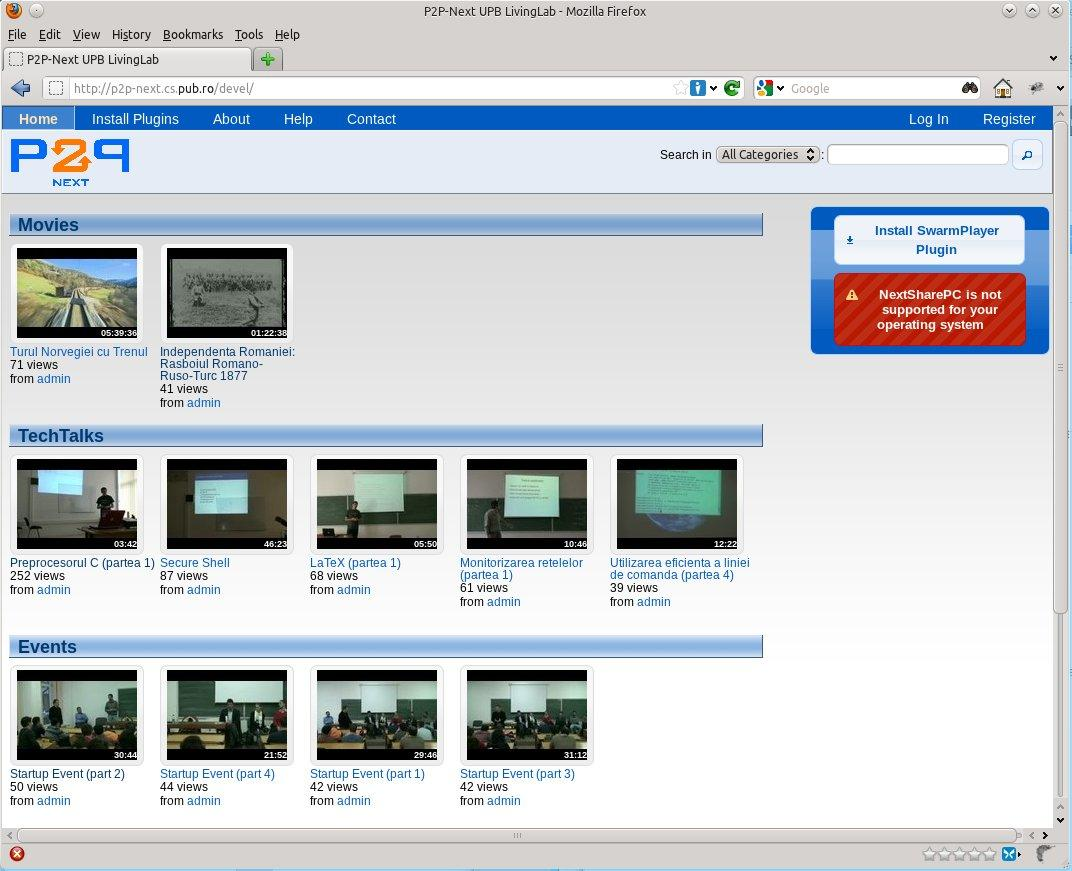
\includegraphics[width=\columnwidth]{img/living-lab-site.jpg}
  \end{center}
  \caption{UPB Living Lab Site -- An Implementation of P2P-Tube}
  \label{fig:living-lab-site}
\end{figure}

We are using P2P-Tube in our university for P2P-Next Living Lab Site (see Figure \ref{fig:living-lab-site})  as a test bed for the Next-Share technology.

\subsection{Web Application Front End}
\label{subsec:front-end}

The front end of P2P-Tube provides an interface with the users of the platform. Today more and more applications are migrating from a classical desktop interface to a web interface. For instance, applications like Microsoft Office started to appear on the cloud, providing a web interface; one popular example is Google Docs. Besides this new trend, Next-Share content delivery platform was successfully implemented in browsers by P2P-Next. So implementing P2P-Tube as a web platform came as a natural choice.

Because almost any hosting provider offers a standard LAMP stack, we decided to cope with such a configuration. LAMP stands for Linux, Apache, MySQL, PHP, the technologies which is based on. We tested P2P-Tube on Apache web server, but it should work well on others.

P2P-Tube server side application is implemented in \textbf{PHP} which is one of the most popular programming languages for this purpose. To facilitate development we decided to use \textbf{CodeIgniter} \cite{code-igniter} open-source framework. Thanks to this framework the platform uses a \textit{MVC (Model-View-Controller)} design pattern, which separates the user interface part (View), from the data stored (Model) under the rule of the Controller.

Our implementation uses a \textbf{MySQL} database, but CodeIgniter abstracts the interface with the database, so porting our platform for a different SQL technology such as PostgreSQL should be easy.

As a web application, on the client side P2P-Tube uses HTML, CSS and JavaScript. As stated before SwarmPlayer only works with browsers that support HTML5. We decided to use jQuery \cite{jquery} as a JavaScript framework to ease development on the client side programming. We developed a jQueryUI \cite{jqueryui} widget which is used to control video playing with features like play, pause and stop buttons, time progress slider, volume control etc.. This widget is detailed in Subsection \ref{subsec:video-widget}.

The web application currently uses two models. \textbf{\texttt{videos} model} is an interface to the database for accessing information about video assets. \texttt{videos} table contains on each row data about a video asset. \texttt{videos_comments} stores each video comment created by an user on a row. Both videos and comments can be voted with like or dislike. Methods for returning detailed information about a video, for returning \textit{video summaries} and for searching in the videos set are implemented here. Video summaries are lists of video assets, with brief information about each one. For instance, \texttt{get_videos_summary} method can create a list of videos from a specific category, uploaded by a specific user, within a defined range described as offset and count and ordered in a specific way. Methods for adding and retrieving comments for voting or for incrementing the number of views for a video are also available here.

\textbf{\texttt{users} model} is an interface to the database for accessing information about users. \texttt{users} table stores on each row data about a registered user, including its user name, its password SHA1 hash, its e-mail and profile information such as gender, country, city, birth date etc.. Authentication information, authentication method (internal, with LDAP or with OpenID) and user preferences are also stored in this table. When signing in with OpenID, \texttt{users} table is joined with \texttt{users_openid} table which maps OpenID URLs with rows from \texttt{users} table. After registration, new users have to confirm their e-mail address by providing an activation code received on that address. Unactivated users with their activation codes are stored in \texttt{users_unactivated}. User activity is logged in \texttt{users_actions} table. This kind of information can be used to ensure that an user votes a comment or a video only one time during a day, but user history can also be tracked here.

\texttt{users} model methods can be used to check authentication credentials, to register new users, to activate accounts, to send password recovery e-mails and to modify user data. Column \texttt{auth_src} from \texttt{users} table identifies the authentication method used by the user. If internal authentication is used the password entered by the user is hashed with SHA1 and checked against the hash from \texttt{password} column. For LDAP authentication this field is NULL, because \texttt{users} model connects to an LDAP server for logging in. For authentication through OpenID, \texttt{users} model uses a third-party library developed by JanRain Inc. \cite{janrain-openid} which implements OpenID protocol.

Pages are organized around a few controller classes. \textbf{\texttt{catalog} controller} manages web pages that help users explore video assets. \textbf{Index page} shows the five most \textit{hottest} video assets from each category which are the newest and the most appreciated ones. The appreciation score is calculated as the number of views plus the number of likes minus the number of dislikes, so a video with a greater appreciation score is more appreciated. \textbf{Category page} permits users to explore video assets by category. Videos can be ordered alphabetically, by upload date or by showing the hottest first.

\textbf{\texttt{video} controller} manages the \textbf{watch page} were users can play a video asset with one of the two Next-Share plugins and the video widget presented in Subsection \ref{subsec:video-widget}. Commenting and voting mechanisms are also implemented into this controller through AJAX, such that when using this facilities the web page is not refreshed interrupting video playing.

\textbf{\texttt{user} controller} is used for user management. \textbf{\texttt{login} method} controls a web page which permits users to sign in with their user name and password or by providing an OpenID. Tree buttons for Yahoo!, Google and myOpenID ease authentication through OpenID with this services. \texttt{login} method checks authentication credentials by using \texttt{users} model and sets a new session in a cookie if authentication succeeded. To delete the session and sign out, \texttt{logout} method is used. \textbf{Registration} and account activation pages are managed by the same controller and logged in users can access \textbf{account page} to change account and profile information or to change their password. To verify that a real person applied for an account, a CAPTCHA is provided on the registration page. Users can see each other's profile through the \textbf{profile page} where one can also see what videos that user uploaded.

The platform provides a way to load static HTML as page content through \textbf{\texttt{article} controller}. The HTML is loaded from \textit{``application/views/article/$<$language$>$/$<$article_name$>$.php''} when URL \textit{``article/$<$article_name$>$''} is accessed. \textit{$<$language$>$} is the name of the current language set in \textit{``application/config/config.php''}. CodeIgniter's URI routing feature can be used in order to have a different URL for an article. In the default configuration of the P2P-Tube site there are four articles used: \textit{Install Plugins}, \textit{About}, \textit{Help} and \textit{Contact}. All of them use URI Routing in order to have a friendlier address.

CodeIgniter supports running its script from the command line. \textbf{\texttt{admin_cli} controller} implements a few methods that can be used by system administrators exclusively from the command line. Database cleanup methods are currently implemented here, which can be conveniently called as cron jobs.

Some parts of a web page are common to more than one page. This include headers, menus, footers, side parts with optional information etc.. All these components are implemented as \textbf{views} and are loaded within the controller of each page. \textbf{\texttt{header} view} renders the top of a web page and includes a menu, a logo, information about the logged in user if required and a search box that help users search video assets, described in Subsection \ref{subsec:searching}. \textbf{\texttt{footer} view} renders the bottom of a web page and typically contains copyright information or links. Common HTML tags like those found into head tag can be easily loaded by using views \textbf{\texttt{html_begin}} and \textbf{\texttt{html_end}}. View \texttt{html_begin} is used with \textbf{\texttt{Html_head_params} library} to load CSS files, JavaScript files, set the page title and add meta data.

\subsection{Searching Video Assets}
\label{subsec:searching}

As stated before the default user interface of the platform provides a search box in the page header along with an options list for narrowing results to a specific category.

The search functionality depends on MySQL Full-Text functions \cite{mysql-fulltext}, thus the search query language is similar. Two modes of full-text searching are used from MySQL: natural language full-text search and boolean full-text search. 

\textit{Natural language full-text search} allows users to enter space separated keywords that are matched against table rows. Searching is performed only in table columns that are indexed for full-text search, so we are indexing \texttt{title}, \texttt{description} and \texttt{tags} columns from \texttt{videos} table. What MySQL calls natural language is in fact vector space search, which calculates the relevance of each result row against the query with some variation of \textit{tf-idf} formula \cite{tf-idf}, one of the most popular used in information retrieval. This kind of searching performs well on our video set of about 120 items. However, natural language search mode has some problems. For instance, any word shorter than four characters is not indexed, so a query like \textit{``let it be''} or \textit{``git c repo''} wouldn't retrieve anything. Also, wild cards, quotations and boolean operators like \textit{and}, \textit{or}, \textit{not} are not supported.

To handle this problem P2P-Tube's search feature also uses MySQL's \textit{boolean full-text search} functions. This mode allows users to enter special characters at the beginning of the keyword from the search query. For example $+$ and $-$ operators indicate if a word is required to be present or absent, respectively, in the results. A full reference of the operators supported can be found in MySQL documentation \cite{mysql-boolean-search}. Boolean search mode is only used when at least one of this operators is present in the search query, otherwise natural search mode is used. Boolean search mode offers a little bit more flexibility to the user, but on the other hand it has a big disadvantage, results are not ordered by their relevance. Instead of assigning a relevance score for each row, this mode adds one for each match of a column and zero otherwise. We weighted columns differently to mark their importance. We mark \texttt{title} as the most important column of the \texttt{video} table with respect to searching, by weighting it with 50\% of the total weight. \texttt{tags} column gets 30\% and description gets 20\%. So if a query matches against the title, 0.5 instead of 1 is added to the relevance, if tags matches, 0.3 is added and if description matches, 0.2 is added.

Like natural language mode, boolean mode also skips words with less than 4 characters, so in our implementation we also search for word fragments in the indexed columns. To support this we use the SQL keyword \texttt{LIKE} along with strings of words containing character \texttt{\%} at the beginning and at the end. If such fragments are matched they affect very little the relevance because the weights of matching columns \texttt{title}, \texttt{tags} and \texttt{description} are very small, being 25\%, 15\% and 10\%, respectively. So, a query string \textit{``let it be''} will match a Beatles' video with the same name, but will also match videos containing \textit{``letter''}, because \textit{``let''} from the query is a fragment of \textit{``letter''}.

For our small video set the search feature performs well without any performance issues. For future work we are planning to use more advanced search tools such as Lucene or Solr from Apache Software Foundation.

\subsection{Video Widget}
\label{subsec:video-widget}

Next-Share browser plugins do not provide an user interface to control and monitor playing of video assets. Users need at least a play button in order to start watching. However, browsers typically offer play controls for HTML5 video tags, but their functionality is limited and depends on the browser, making video tags look browser dependent. While SwarmPlayer has some kind of user interface by using HTML5, NextSharePC is based on VLC browser plugin, which does not come with any interface.

\begin{figure}[h]
  \begin{center}
    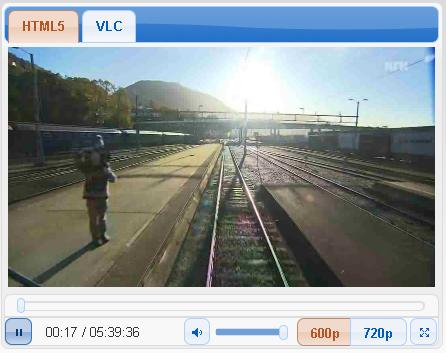
\includegraphics[width=\columnwidth]{img/nsvideo-widget.jpg}
  \end{center}
  \caption{\textit{NS Video} Widget}
  \label{fig:nsvideo-widget}
\end{figure}

We decided to create a browser widget, based on jQueryUI that can be used with both Next-Share plugins. Besides this functionality our widget, named \textbf{NS Video} (Next-Share Video), can be used without Next-Share technology for playing ``pure'' HTML5 videos and to control ``pure'' VLC plugins. A snapshot of the widget be seen in Figure \ref{fig:nsvideo-widget}. It was designed as a separate component of P2P-Tube and it can be used in any other web application, just like any jQueryUI widget. It is a widget combined from other standard jQueryUI widgets like buttons, sliders and check boxes and it uses jQueryUI's CSS framework.

HTML5 triggers events for the video tag, so for example when the video finishes playing an event is triggered. This simplified a lot the widget implementation for SwarmPlayer. This was not the case with NextSharePC, which uses VLC and does not trigger any events. To solve this problems we used JavaScript timers which check plugin's state periodically and applies the appropriate actions.

The widget contains two \textit{interfacing objects} (which have the same interface), one for HTML5 (named \texttt{html5}) and one for VLC (named \texttt{vlc}). With this two objects the widget's interfacing with to the two different video technologies is simplified. If a future extension for another technology, other than HTML5 and VLC, is required, a developer only needs to implement the methods of a new interfacing object.

\subsection{Content Ingestion Back End}
\label{subsec:back-end}

Content Ingestion Server is written in Python, mainly because of the need of using threads. A master thread takes the role of a producer by receiving requests from clients and submitting them to a job queue. The consumer is a worker thread which gets jobs from the queue and executes them, using a first-come first-served servicing policy. If the queue is empty the worker waits without blocking until a new job is available. 

Client requests are received by the master through a RESTful web service. This functionality was implemented with \textbf{Web.py} \cite{webpy}, a lightweight web framework for Python. Simpler messages, like the one which requests CIS's load are implemented with HTTP GET methods, but more complex ones which require structured data format use POST methods. The posted data is encoded with JSON (JavaScript Object Notation) which allows messages to be formated as an imbrication of lists and dictionaries.

CIS implementation depends on NextShareCore library for the functionalities of creating and seeding torrent files. As stated before this library is also written in Python, so that was another motivation for writing CIS in this programming language. NextShareCore provides an efficient implementation of seeding by using threads.

Besides creating torrents and seeding, a content ingestion job also needs to transfer locally raw video files from the web server, to transcode them to destination formats, to extract image thumbnails and to transfer back torrent files and image thumbnails to the web server. For this purpose all this features use a pluggable interface. In \texttt{api} package, file \texttt{base.py} contains this interfaces detailed below:

\begin{itemize}
 \item \textbf{\texttt{BaseFileTransferer}} abstracts file transfers between CIS and web server.
 \item \textbf{\texttt{BaseTranscoder}} abstracts video asset transcoding, so raw video files can be transcoded to destination formats by using an implementation of this base class.
 \item \textbf{\texttt{BaseThumbExtractor}} abstracts image thumbnails extraction from video assets. Multiple extraction policies can be provided. A thumbnail can be extracted from a specific position from the video given in seconds, from random a position or summary thumbnails can be extracted, where a series of thumbnails by taking several snapshots are captured.
 \item \textbf{\texttt{BaseAVInfo}} abstracts a tool for retrieving information about a video asset. Currently this interface can be used to get the duration of a video.
\end{itemize}

Developers can extend this interface classes with their own implementation. In CIS configuration file (\texttt{config.py}) system administrators can choose between several alternative implementations of a feature. Currently file transfers are done with FTP (File Transfer Protocol) \cite{ftp} with class \texttt{FTPFileTransferer} which extends \texttt{BaseFileTransferer}. Standard FTP Python libraries are used for this purpose. FTP uses two ports for communication between client and server, one corresponding to the control channel, the other one to the data channel. The control channel could transfer sensitive information, thus TLS (Transport Layer Security) \cite{tls} is used for encryption. Developers are encouraged to implement other alternative protocols for file transfers. For example, we are planning an rsync \cite{rsync} implementation which recovers better from failures and checks data integrity. Despite the fact that FTP is less advanced than rsync, we decided to implement it because of its popularity.

Our \texttt{BaseTranscoder} implementation, \texttt{FFmpegTranscoder}, uses \textit{FFmpeg} \cite{ffmpeg} a software solution for recording, converting and streaming audio and video. Transconding is possible between almost any formats, by using third-party libraries. Being written in C, CIS forks a new process when using FFmpeg, and creates a pipe for monitoring standard output and standard error. Porting P2P-Tube to Windows should be easy because FFmpeg also works on this operating system.

FFmpeg can also be used for extracting thumbnails, so we used the same software for implementing \texttt{FFmpegThumbExtractor}, which extends \texttt{BaseThumbExtractor}. Information about a video asset can be obtained with \texttt{FFprobeAVInfo}, an implementation of \texttt{BaseAVInfo} base class, which uses ffprobe an utility from FFmpeg software package.

\textbf{CIS-LB} (CIS -- Load Balancer) usually lays on the same machine with a web server and also communicates with it via web services. Thus, we implemented CIS-LB in Python, using Web.py as CIS. Messages received from a web server are forwarded to a CIS from the pool by using a load balancing policy. Policies are implemented as pluggable interfaces exactly as features of CIS are. Three possible policies can be used:

\begin{itemize}
 \item \textbf{Random}: choose a random CIS from the pool and forward the request from web server to it.
 \item \textbf{Optimum}: send a get load request to each CIS, calculate which one is the least loaded and forward the request from web server to it.
 \item \textbf{Randomized Suboptimal}: choose $k$ random CIS machines, send a get load request to each one, calculate which one is the least loaded and forward the request from the web server to it.
\end{itemize}

The \textit{optimum policy} is slower because it must wait until all CIS machines respond to get load request, so although it finds the best solution it does not scale for systems with a big number of CIS machines. This policy is recommended for small scale systems. The \textit{random policy} is the fastest, but it doesn't found the best solution, but it loads each CIS machine with equal probability, providing a good load balancing. It is recommended for big systems.  \textit{Randomized suboptimal policy} is a compromise between optimum policy and random policy and is recommended for medium sized systems. The choice between the three policies not only depends on the number of CIS machines from the system, but also on the size of the raw video files that need to be processed.

\subsection{Front End and Back End Communication}
\label{subsec:communication}

The web server needs to communicate with Content Ingestion Server, whether or not through a CIS Load Balancer (CIS-LB), by sending a content ingestion request. By using a web service for this communication  implementation overhead is reduced. Sending HTTP requests from the PHP web server application is much more easy then creating a custom new protocol. The same applies at the other communication point, the Python server, where requests are received by Web.py framework, which makes HTTP methods processing extremely easy.

If another video platform decides to use our solution based on CIS machines, interoperability is simplified by using web service interfaces, no matter what programming language is used for web server application.

\subsection{The Choice for the Web Service Type}
\label{subsec:web-service}

Our choice between a SOAP web service and a simple RESTful web service was based on our needs. We wanted to make a server with a low communication overhead and SOAP has the disadvantage of consuming more computational resources when processing requests. Our messages that need to be passed through different services have a simple structure. 

The \textit{get load request} does not have any parameters, so a simple HTTP GET request is sufficient and any extra data transmitted as XML with SOAP is redundant.

\textit{Content ingestion request} is a message with a greater complexity. The name of the uploaded file located on the web server needs to be transmitted, along with video formats information such as containers, codecs used, resolutions, frame rates, aspect ratios, audio sampling rates and bit rates. All these information would fit well as parameters in a SOAP message. However encoding them in a JSON seemed to be a much simpler solution. Both PHP and Python offer functions that convert their primitive types and data structures, like lists and dictionaries, into JSON strings. XML messages have a greater verbosity comparing to JSON messages. Features like XML tag attributes are not required for our application.

We expect web servers and their CIS Load Balancers to know CIS machines in advance. So there is no need for discovery services that could provide contact information for new CIS machines. This would reduce administrative control and would raise security concerns like discovering malicious CIS machines. So there is no need for service discovery features like UDDI from SOAP ecosystem.

Services functionality does not need to be described because it is expected to be known in advance by the client application, so SOAP's WSDL feature is not needed.

The simplicity of our web services and our need for a low communication footprint suggested us to use a RESTful web service with JSON encoded information when the POST method is needed. SOAP extra features like WSDL and UDDI are not required for our application, giving us another reason to exclude it as a candidate.